\documentclass[a4paper]{article}

%% Language and font encodings
\usepackage[swedish]{babel}
\usepackage[utf8x]{inputenc}
\usepackage[T1]{fontenc}

%% Sets page size and margins
\usepackage[a4paper,top=3cm,bottom=2cm,left=3cm,right=3cm,marginparwidth=1.75cm]{geometry}

%% Useful packages
\usepackage{amsmath}
\usepackage{graphicx}
\usepackage[colorinlistoftodos]{todonotes}
\usepackage[colorlinks=true, allcolors=blue]{hyperref}
\usepackage{titling}

\usepackage{fullpage}
\usepackage{setspace}
\usepackage{mathrsfs}
\usepackage{amsfonts}
\usepackage{chngcntr}

\usepackage{titlesec}
\setcounter{secnumdepth}{4}
\titleformat{\paragraph}
{\normalfont\normalsize\bfseries}{\theparagraph}{1em}{}
\titlespacing*{\paragraph}
{0pt}{3.25ex plus 1ex minus .2ex}{1.5ex plus .2ex}

\title{Maskininlärning i framtidens elnät}
\author{Emil Arvidsson}
\date{\today}

\begin{document}

%Skapa en framsida
\begin{titlepage}
\doublespacing
\centering 
\vspace{2 cm}
% Detta gör ett 3 cm långt mellanrum till nästa rad
{\LARGE {\bf Maskininlärning i framtidens elnät}}  \\
\vspace{1 cm}
% Skriv in titeln
\centering 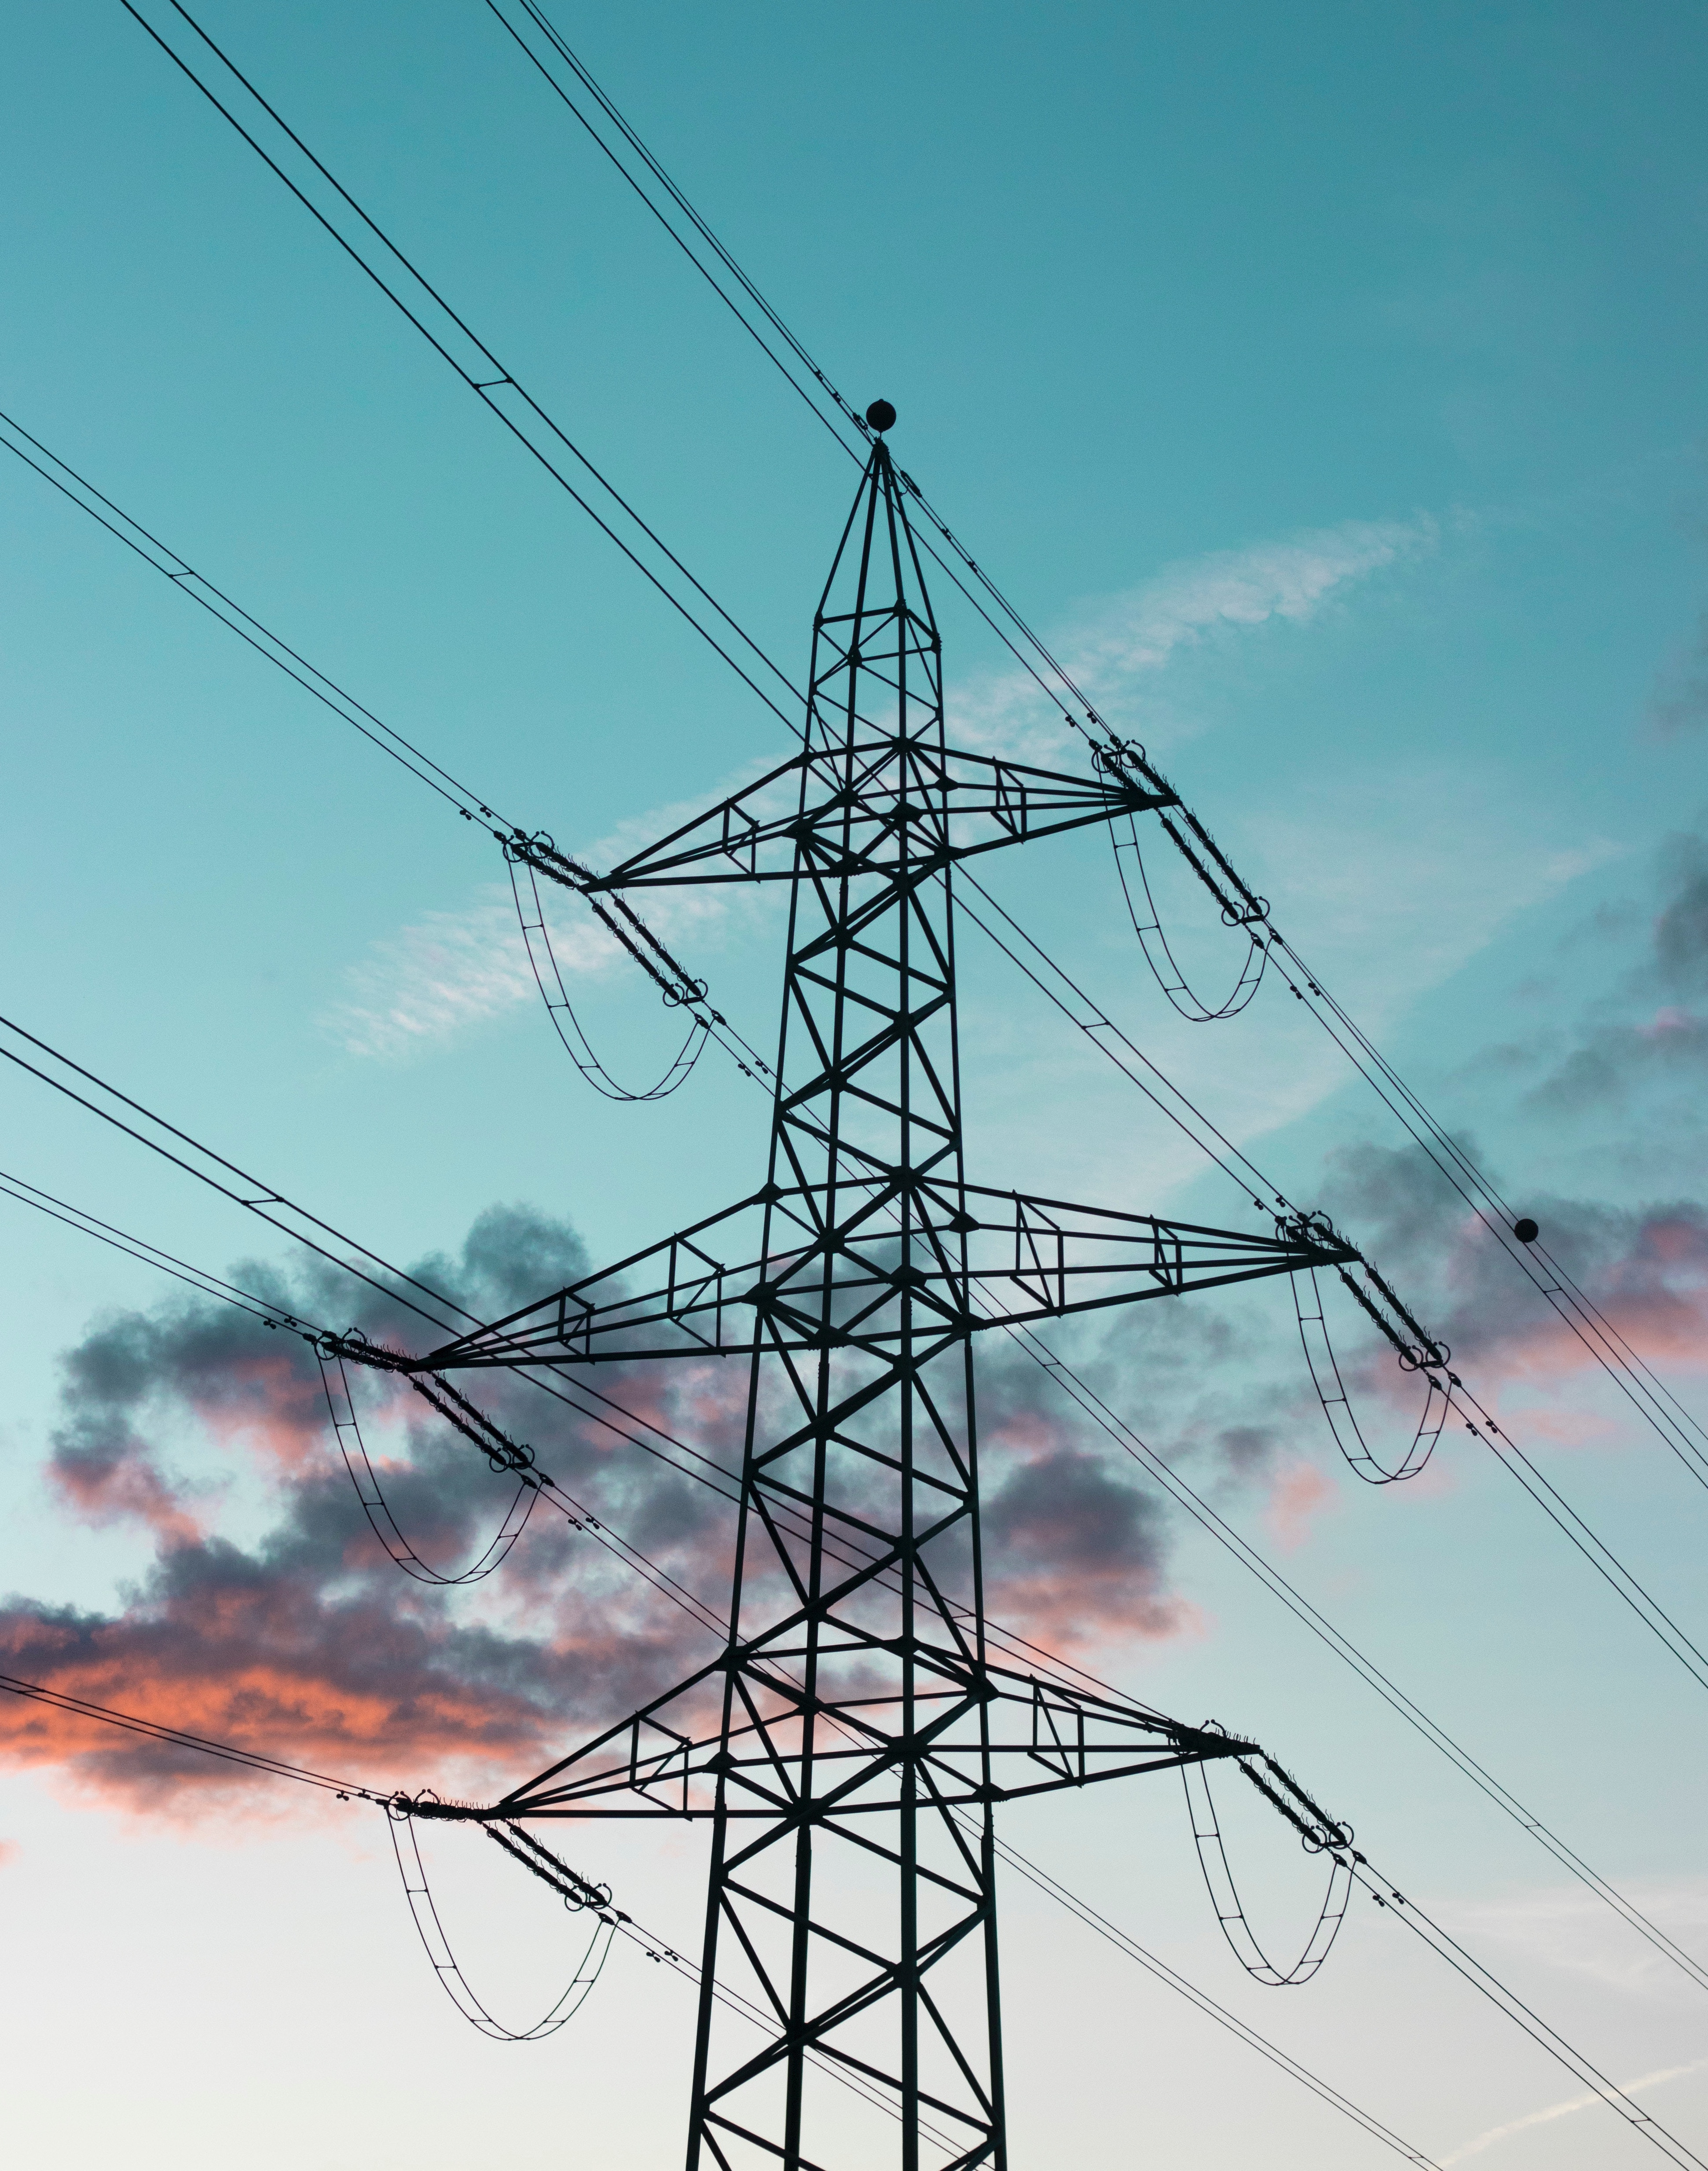
\includegraphics[scale=0.08]{powerline.jpg} \\	
\vspace{1 cm}
{\bf Skriven av}:\\ Emil Arvidsson\\        
% Skriv era namn 
\vspace{3 cm} 
% Detta gör ett 3 cm långt mellanrum till nästa rad


Uppsala \\ 2018-04-19
% Skriv in datumet
\end{titlepage}


\clearpage










\begin{abstract}
Your abstract.
\end{abstract}

\clearpage

\tableofcontents

\clearpage

\section*{Begrepp}

\begin{description}
\item \textbf{Input} - Information som matas in i ett program/algoritm.
\item \textbf{Output} - Information som ges ut från ett program/algoritm.
\item \textbf{Data} - Information.

\end{description}

\clearpage

\section{Inledning}

Här ska det stå något kul!

\subsection{Syfte och frågeställningar}
I och med att teknik som artificiell intelligens och maskininlärning blir allt mer vanligt i alla branscher ställs nu även frågan hur elnätsbranschen ska kunna använda dessa tekniker. För att kunna ta ställning till var man bör börja är det nyttigt att utreda var potentialen finns och vilken teknik som är lätt att implementera. Därför kommer denna rapport behandla följande frågeställningar:

\begin{itemize}
	\item Vilka förluster finns i elnätet som konsekvens av brister i system och underhåll? \\
    \item Var finns det potential att implementera maskininlärning för att förbättra systemet?
\end{itemize}


\subsection{Avgränsningar}
Rapporten kommer inte att ta någon hänsyn till ekonomiska aspekter utan enbart fokusera på de tekniska möjligheterna. Ekonomiska drivkrafter kan dock komma att spela in vid bedömningen av var potentialen ses som störst. Rapporten kommer endast beröra implementering i det svenska elnätet men tekniker som används på andra platser i världen kan komma att spela roll. 

Eftersom det finns många delar av elnätet kommer denna rapport att avgränsa sig till att endast behandla maskininlärning för att prediktera last och förutse fel, slitage och underhåll.

För att avgränsa ytterligare kommer endast lösningar som inte innebär större ingrepp i det befintliga nätet behandlas. Det vill säga att mjukvaruförändringar och mindre hårdvarutillägg kommer vara i fokus.

Endast transmission kommer behandlas av denna rapport. Dvs, rapporten bortser från de delar av enlätet som innebär steget mellan nät och slutkonsument och tekniska aspekter rörande elproduktion.




\clearpage


\section{Huvuddel}

\subsection{Vad är maskininlärning?}

\subsubsection{Definition}
Maskininlärning definieras enligt Kevin P. Murphy, i Machine Learning: A Probabilistic Perspective (2014), som en uppsättning metoder som automatiskt kan upptäcka mönster i data och använda dessa upptäckta mönster för att sedan förutse framtida data, eller annan sorts beslutsfattande givet en osäkerhet.

\subsubsection{Historia}


\subsubsection{Tekniker och tillvägagångssätt}

Maskininlärning kan enligt Murphy kategoriseras i tre kategorier som beskriver hur teknikerna lär sig av sin omgivning. Dessa är "Supervised machine learning", "Unsupervised machine learning" och "Reinforcement machine learning". Av dessa är "Supervides machine learning" den mest använda typen. Nedan följer beskrivningar av de två förstnämnda enligt Murphy samt den sistnämnda enligt XXX LÄGG TILL KÄLLA!!

\paragraph{Supervised machine learning}

Som namnet avslöjar handlar "Supervised machine learning" om övervakad och "ledd" maskininlärning ("Övervakad maskininlärning"). Algoritmen läser av data men får även reda på vad en viss typ av data betyder/indikerar. Genom att ge en sådan algoritm tillräckligt mycket grunddata med "facit" kan den sedan prediktera vad ny data betyder/indikerar utan givet "facit". Denna maskininlärningsmetod lämpar sig framför allt för klassifikation eller regression. 

Klassifikation innebär att algoritmen kan avgöra vad in-datan betyder och utföra ett visst uppdrag beroende på vilken klass den har identifierat. Ett exempel är analys av effektkurvor från mätdata hos elledningar. Algoritmen skulle kunna avgöra om en serie mätdata är normal eller avvikande och bör avge ett larm till operatör. Detta är vad som kallas "binär" klassificering, d.v.s. algoritmen kan ge värdet 0 eller 1 och är den simplaste typen av klassificering. En mer avancerad algoritm skulle dock t.ex. kunna göra fler klassificeringar och kunna avgöra utifrån es serie mätdata om elnätet fungerar normalt, avvikande av typ 1, avvikande av typ 2 eller avvikande av typ 3. Därpå utföra en lämplig åtgärd, förslagsvis reglera mängden kapacitiv och induktiv last. Dessa klassificeringar benämns som "multiclass"-klassificering (t.ex. svag, normal, stark) eller "multi-label"-klassification (t.ex. stark, lång, varm). För att algoritmen ska kunna ha någonting att förhålla sig till behöver det väljas ut vissa parametrar som faktisk det går att dra en slutsats utifrån, vilket inte nödvändigtvis är lätt. Klassificering används snarare för att hantera redan inkommen data än för prediktering.

Regression i sin tur är likt klassificering men algoritmen utför här vad som kan liknas med kontinuerlig klassifikation istället för diskret sådan. Det enklaste exemplet skulle vara linjär kurvanpassning för tvådimensionell data. Regressionsanalysen kan däremot användas för annan anpassning och för oändliga dimensioner i teori. Regression lämpar sig, till skillnad från klassificeringen, för prediktering av kommande data. Exempel skulle kunna vara att förutse framtida aktiepriser eller väderförhållanden.


\paragraph{Unsupervised machine learning}

"Unsupervised machine learning" ("Oövervakad maskininlärning") skiljer sig från den tidigare nämnda "Supervised learning" genom den inte särskilt förvånande aspekten att den är så kallad oövervakad, som namnet antyder. Vad obevakad innebär är inte nödvändigtvis att algoritmen kör helt utan någon sorts mänsklig kontroll. Obevakad syftar snarare på att algoritmen inte kräver någon input från en människa utan endast läser data och klarar av att själv bedöma och ge en output utifrån en slutsats som algoritmen helt genererat själv. Med det sagt används inte oövervakad maskininlärning på samma sätt som den övervakade. Målet med den här metoden är att hitta mönster eller kluster i datan. Murphy uttrycker det som att målet inte längre är att hitta \emph{ett} svar utifrån en given parameteruppsättning. Istället ska nu en okänd mängd parametrar jämföras där det sökta svaret snarare är en multivariabel sannolikhetsmodell som berättar vilka data som troligen tillsammans bildar det sökta svaret. Att på det här sättet hitta intressanta strukturer i datan kallas ibland för "knowledge discovery" eftersom algorimen hittar mönster utan att någon människa har berättat vad den letar efter.

Det är inte svårt att komma fram till slutsatsen att oövervakad maskininlärning är en svårare uppgift att ta sig an. Däremot har den många fördelar och kan, enligt Murphy, appliceras i allt bredare kontexter. Han påpekar även att det går att argumentera för att denna typ av algoritm liknar djurs och mänskligt tänkande och tar upp exemplet att om en människa ska lära sig vad någonting innebär kan den inte tillgodogöra sig tillräckligt med information utifrån enskilda parametrar i data, utan måste hantera hela datamängden i sig för att finna alla kombinationer av mönster. I praktiken betyder detta att algoritmer som först måste ges ett "facit" för att fungera genererar relativt lite information, samtidigt som det är en dyr process att tillhandahålla programmet med detta "facit". Därför kan oövervakad maskininlärning ge ett betydligt större informationsutbyte. 


\paragraph{Reinforcement machine learning}




\clearpage



\subsection{Maskininlärning i dagens elnät}

\subsubsection{KulKulKUl}

\clearpage



\subsection{Brister i elnätet}

I alla delar av elnätet finns brister som kan ge förluster, både ekonomiskt men även säkerhetsmässigt. Många av dessa adresseras redan av konventionell teknik medan vissa inte alls går att lösa utan intelligenta system och maskininlärning. Saxena \emph{et al.} (2010) gör denna beskrivning och listar följande som områden i elnätet där det finns potential att utföra arbetet bättre för att få ett mer effektivt elnät.

\begin{itemize}
	\item Allmän drift
    \item Driftkontroll
    \item Systemautomation
    \item Geografisk resursplanering
    \item Prognostisering   
\end{itemize}

Allmän drift syftar på de funktioner som ligger till grunden för ett välmående nät, alltså generellt effektflöde och nätunderhåll. Elnätet bör användas på ett sätt som förhindrar överbelastning på några sträckor i nätet (Bush 2014). Att utföra underhåll på de delar som är susceptibla för slitage är också en nödvändighet för att driva ett elnät utan stora förluster och säkerhetsrisker. Båda dessa punker är något som redan idag behandlas men inte så effektivt som hade kunnat behövas (Saxena et al. 2010). 

Driftkontroll är förmågan att reglera de parametrar som avgör kvalitén och transportförlusterna i elnätet. Exempel på dessa parametrar är effektfaktor, spänningsnivåer och frekvens. Dessa parametrar går inte att alla enskilt optimera samtidigt (Bush 2014), varför ett system som på ett objektivt sätt kan maximera dessa utifrån den kravspecifikation som finns kan förbättra effektiviteten i elnätet.

Systemautomation innebär att systemet själv kan hantera händelser som avviker från den normala driften och begära lämpliga åtgärder. Sådana händelser kan vara väderpåverkan, plötsliga lastförändringar, plötsliga produktionsförändringar, fysiska skador i systemet bl.a. Programmet ska både kunna klassificera vilket fel som har inträffat men också kunna utföra nödvändiga åtgärder för att lösa problemet. Exempel på åtgärder kan vara att leda om strömmen, starta om den berörda systemdelen eller tillkalla reparatörer. 

Geografisk resursplanering avser förmågan att kunna avgöra var el bör produceras och var den bör transporteras och får effekt av två anledinngar. Elgenerationen kommer i allt störra skala från decentraliserade källor som vind- och solkraft. Elen bör också produceras så nära slutkund som möjligt för att undvika transmissionsförluster.


Test test online

test test offline Vad händer? Offlene vadå

\clearpage 



\subsection{Åtgärder med maskininlärning}

\clearpage



\section{Diskussion}

\clearpage



\section{Slutsats}

\clearpage



\section{Litteraturförteckning}


\subsection{How to add Citations and a References List}

You can upload a \verb|.bib| file containing your BibTeX entries, created with JabRef; or import your \href{https://www.overleaf.com/blog/184}{Mendeley}, CiteULike or Zotero library as a \verb|.bib| file. You can then cite entries from it, like this: \cite{greenwade93}. Just remember to specify a bibliography style, as well as the filename of the \verb|.bib|.

You can find a \href{https://www.overleaf.com/help/97-how-to-include-a-bibliography-using-bibtex}{video tutorial here} to learn more about BibTeX.

We hope you find Overleaf useful, and please let us know if you have any feedback using the help menu above --- or use the contact form at \url{https://www.overleaf.com/contact}!

\bibliographystyle{alpha}
\bibliography{sample}

\end{document}